\documentclass[8pt,a4paper]{article}

% --- Geometry ---
\usepackage[margin=0.9cm,top=0.85cm,bottom=0.85cm]{geometry}
\usepackage[utf8]{inputenc}
\usepackage[T1]{fontenc}
\usepackage{lmodern}
\usepackage{microtype}

% --- Graphics & tables ---
\usepackage{graphicx}
\usepackage{booktabs}
\usepackage{tabularx}
\usepackage{multirow}
\usepackage{float}
\usepackage{colortbl}

% --- Math ---
\usepackage{amsmath}

% --- Colors & links ---
\usepackage[dvipsnames]{xcolor}
\usepackage[colorlinks=true,linkcolor=MidnightBlue,urlcolor=MidnightBlue,citecolor=MidnightBlue]{hyperref}

% --- Section formatting (compact) ---
\usepackage{titlesec}
\titleformat{\section}{\normalfont\bfseries\normalsize\color{MidnightBlue}}{\thesection.}{0.4em}{}
\titleformat{\subsection}{\normalfont\bfseries\small\color{MidnightBlue}}{\thesubsection}{0.4em}{}
\titlespacing*{\section}{0pt}{4pt}{1pt}
\titlespacing*{\subsection}{0pt}{2pt}{0pt}

% --- Compact lists ---
\usepackage{enumitem}
\setlist{nosep,leftmargin=1.1em,topsep=0pt}

% --- Header ---
\usepackage{fancyhdr}
\pagestyle{fancy}
\fancyhf{}
\rhead{\scriptsize Milan Viallet --- Albert School B2 BDD}
\lhead{\scriptsize\textbf{Deliverable~2} --- Direction \& Early Results}
\rfoot{\scriptsize\thepage/2}
\renewcommand{\headrulewidth}{0.4pt}

% --- Paragraph ---
\setlength{\parindent}{0pt}
\setlength{\parskip}{1.5pt}

% ======================================================================
\begin{document}

\begin{center}
{\normalsize\bfseries\color{MidnightBlue} Deliverable~2 --- Direction \& Early Results}\\[1pt]
{\scriptsize Sephora Customer Segmentation \quad$\cdot$\quad Milan Viallet \quad$\cdot$\quad April~2, 2026}
\end{center}
\vspace{-4pt}\hrule height 0.5pt\vspace{2pt}

% ======================================================================
\section{A. Retrospection --- Since Grill~1}
% ======================================================================

Three feedback items reshaped the project since Grill~1:
\textbf{(1)} \emph{``PCA kills interpretability''} $\Rightarrow$ removed PCA from clustering; we now cluster on \textbf{46 scaled features} directly (PCA kept only for correlation circle visualization).
\textbf{(2)} \emph{``Too many noisy features''} $\Rightarrow$ classified features into 6 marketing categories, removed 16 non-actionable ones (70 $\to$ 46 features).
\textbf{(3)} \emph{``Track experiments''} $\Rightarrow$ MLflow integration planned next sprint.
\textbf{Scope:} depth-first K-Means with Hierarchical + GMM as comparison baselines.

% ======================================================================
\section{B. Analysis --- Method \& Results}
% ======================================================================

\textbf{Method.} K-Means on $n{=}64{,}469$ customers, 46-dim feature space. Pipeline: transactions $\to$ customer aggregation (RFM + channel + product + behavior) $\to$ drop non-actionable $\to$ median imputation + OHE $\to$ StandardScaler $\to$ K-Means ($k{=}2$--$30$).
\textbf{$k{=}9$} via elbow + silhouette (0.156) + Davies--Bouldin (1.63). Modest silhouette typical for retail behavioral data (0.10--0.25 in literature).

\vspace{-2pt}
\begin{figure}[H]
\centering
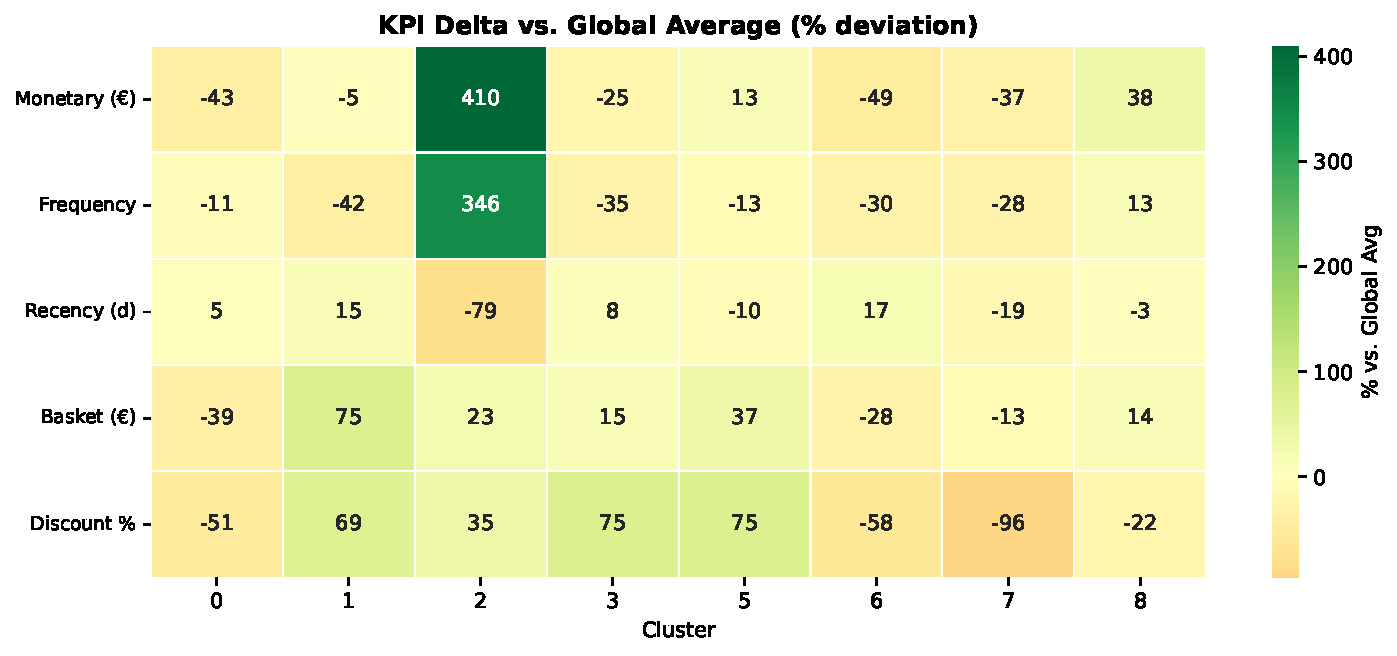
\includegraphics[width=0.88\textwidth,height=4.0cm,keepaspectratio=false]{figures/d2_fig1_kpi_delta.pdf}
\vspace{-2pt}

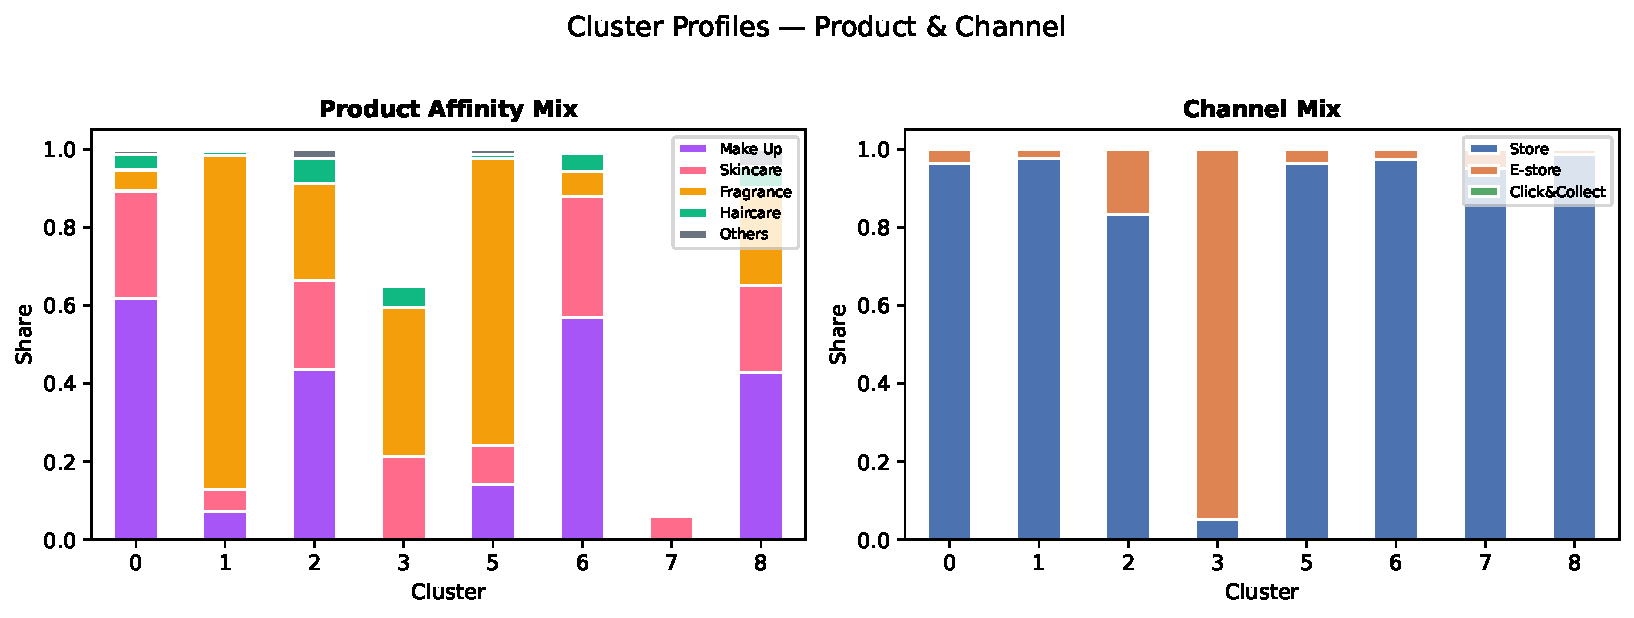
\includegraphics[width=0.88\textwidth,height=3.5cm,keepaspectratio=false]{figures/d2_fig2_cluster_profiles.pdf}
\vspace{-6pt}
\caption*{\scriptsize\textbf{Top:} KPI deviation (\%) vs.\ global avg. \textbf{Bottom:} Product affinity (L) \& channel mix (R) per cluster.}
\end{figure}
\vspace{-8pt}

\subsection{Clusters vs.\ Global Average}

\vspace{-2pt}
\begin{table}[H]
\centering\scriptsize
\setlength{\tabcolsep}{3pt}
\begin{tabularx}{\textwidth}{@{}c r r r r r r l@{}}
\toprule
\textbf{C} & \textbf{\%} & \textbf{Monet.} & \textbf{Freq} & \textbf{Rec.} & \textbf{Bask.} & \textbf{Disc.} & \textbf{Key Insight} \\
\midrule
\rowcolor{gray!8}
\textit{All} & \textit{100} & \textit{\texteuro198} & \textit{3.0} & \textit{111d} & \textit{\texteuro70} & \textit{12\%} & \textit{Global baseline} \\
0 & 30.7 & \texteuro114 & 2.7 & 117d & \texteuro43 & 6\% & Low-spend Make~Up store-only \\
1 & 10.6 & \texteuro189 & 1.8 & 128d & \texteuro122 & 20\% & High-basket Fragrance gifters \\
\rowcolor{green!6}
2 & 5.9 & \texteuro1{,}010 & 13.4 & 24d & \texteuro85 & 16\% & \textbf{VIP loyalists (49\% Gold)} \\
3 & 8.4 & \texteuro148 & 2.0 & 120d & \texteuro80 & 20\% & Digital-first (95\% e-store) \\
5 & 19.9 & \texteuro223 & 2.6 & 101d & \texteuro95 & 20\% & Mid-value Fragrance fans \\
6 & 20.7 & \texteuro100 & 2.1 & 130d & \texteuro50 & 5\% & Dormant low-engagement \\
7 & 2.9 & \texteuro125 & 2.2 & 90d & \texteuro61 & 0\% & Others-axis, zero discount \\
8 & 1.0 & \texteuro273 & 3.4 & 108d & \texteuro79 & 9\% & High-freq multi-brand \\
\bottomrule
\end{tabularx}
\end{table}
\vspace{-6pt}

C2 (5.9\%) = \textbf{5.1$\times$} global monetary, 49\% Gold. C3 confirms digital-native hypothesis (95\% e-store $\neq$ 80\% store base). C4 (4 customers) excluded as noise.

% ======================================================================
\section{C. Evaluation \& Confidence}
% ======================================================================

\textbf{Done:}
\textbf{(1)} Internal metrics --- Silhouette\,=\,0.156, DB\,=\,1.63, CH\,=\,6{,}471;
\textbf{(2)} UMAP 2D shows clusters in visually distinct regions;
\textbf{(3)} Business coherence --- every cluster maps to a plausible marketing narrative (table above);
\textbf{(4)} Correlation circle confirms no remaining redundant pairs ($\cos{>}0.90$) after feature refonte.

\textbf{Planned:}
\textbf{(1)} Kruskal--Wallis tests on all KPIs for statistical significance;
\textbf{(2)} Bootstrap stability ($n{=}50$, ARI $>0.80$ target);
\textbf{(3)} Agglomerative + GMM comparison to rule out algorithm artifacts.

\textbf{Weaknesses:}
\textbf{(1)} Cluster~4 (4 customers) = micro-cluster artifact. Will absorb or flag.
\textbf{(2)} Age imputed with median for 13\% missing --- may flatten age-based differentiation. Fix: \texttt{IterativeImputer} with RF.

% ======================================================================
\section{D. Roadmap --- Path to Finish}
% ======================================================================

\vspace{-2pt}
\begin{table}[H]
\centering\scriptsize
\begin{tabularx}{\textwidth}{@{}c l X c@{}}
\toprule
\textbf{\#} & \textbf{Task} & \textbf{Description} & \textbf{ETA} \\
\midrule
1 & Pipeline cleanup & Remove PCA, integrate MLflow tracking & Apr 3 \\
2 & Notebook refonte & End-to-end clean notebook & Apr 4 \\
3 & Algorithm comparison & Hierarchical, GMM; compare metrics & Apr 5 \\
4 & Validation & Kruskal--Wallis + bootstrap stability & Apr 6 \\
5 & Personas + Impact & Name segments, persona cards, CLV delta, prioritization matrix & Apr 7--8 \\
6 & Final delivery & Polished PDF + code + recommendations & Apr 9 \\
\bottomrule
\end{tabularx}
\end{table}
\vspace{-4pt}

\textbf{Business value:} CLV gap per segment $\to$ estimate revenue uplift from targeted campaigns. Example: moving C6's basket from \texteuro50 to \texteuro70 (+40\%) across 13{,}368 customers $\times$ 2.1 visits = \textbf{\texteuro560K incremental annual revenue}.

\vfill
\begin{center}
\scriptsize\color{gray}\itshape Work in progress. All numbers from pipeline output (main branch, April~2, 2026).
\end{center}

\end{document}
